\section{Experiments}
\label{sec:expt}

\subsection{Testbed}

\subsubsection{CoNLL benchmark}

The CoNLL dataset ~\cite{Hoffart2011} contains 1,393 articles with
about 34K mentions, and the standard performance metric is
mention-averaged accuracy.  The documents are partitioned into train,
test-a and test-b.  Most authors report performance on the subset of
231 test-b documents with 4,483 linkable mentions.

\subsubsection{TAC-KBP benchmark}

The TAC KBP datasets \cite{TAC2011,TAC2012} include 2,226 mentions
(2012) and 2,250 mentions (2011), of which roughly half are linkable
to the reference KB.  The competition evaluation includes $\NIL$
entities; participants are required to cluster $\NIL$ mentions across
documents so that all mentions of each unknown entity are assigned a
unique identifier.  For these datasets, we report in-KB accuracy,
overall accuracy (including $\NIL$ mentions), and the competition
metric $B^{3+} F_1$.


\begin{table*}
  \centering
  \begin{tabular}{l|l|r}
    System                 &  Alias-entity mapping  & In-KB accuracy \\
    \hline
    \newcite{Chisholm2015} & YAGO                   & 88.7\% \\
    Plato \cite{Lazic2015} & (Proprietary)          & 86.4\% \\
    Single link            & Base                   & \todo{87.1\%} \\
    Our baseline           & Base+HP                & 90.2\% \\
    Attention              & Base+HP                & 91.5\% \\
    \hline
    Attention              & Only HP                & *92.84\% \\
    \newcite{Pershina2015} & Only HP                & *91.77\%
  \end{tabular}
\caption{CoNLL test-b evaluation for recent competitive systems and
  our models.  Accuracies obtained with alias-entity maps having very
  low average ambiguity are marked with `*'.  For details of
  alias-entity maps, see Table~\ref{tab:AliasTable} and text.}
 \label{table:conll_results} 
\end{table*}


\begin{table*}
  \centering
  \begin{tabular}{l|r|r|r|r|r|r}
    Alias-entity & Mention &   Gold & Unique & Average   & Baseline & Attention \\
    map          & recall  & recall &        & ambiguity & accuracy & accuracy \\
    \hline
    Base     & 4318 & 91.3\%, 4095 & 1055   & 55.7      & 88.29\%   & 89.49\%  \\
    Base+HP  & 4477 & 99.9\%, 4477 & 955    & 60.9      & 90.23\%   & 91.50\%  \\
    *Only HP & 4477 & 4476   & 1224   & 13.3      & 92.10\%   & 92.84\%  \\
    Base+HP+YAGO & 4477    & 4477   & 879    & 79.4      &          &           
  \end{tabular}
  \caption{Effect of alias-entity mapping tables.  CoNLL, test-b
    fold, 4483 gold mentions.  Mention recall is the number of
    mentions with at least one known entity; gold recall is the number
    of cases where the gold entity was included in the candidates.
    Unique cases have only one candidate.  Ambiguity is averaged over
    mentions with at least one candidate.}
  \label{tab:AliasTable}
  % old KG
\end{table*}





\subsubsection{Local and pairwise scores}
\label{sec:expt:features}

Our baseline system is similar to Plato \cite{Lazic2015} in terms of
design and accuracy.  For each candidate $c$ for mention $i$, it emits
a posterior distribution $p_i(c)$.  The baseline system does not have
an explicit coherence model; however, it does capture some coherence
information indirectly, because referrent phrases are included as
string features.  For standardized comparison we limit ourselves to
candidates proposed by the baseline system.

\paragraph*{Scores for single-link model:}
In the \emph{single link} model, we simply set the local score for
mention $i$ and candidate $c$ to $s_i(c) = \ln p_i(c) - \ln (1 -
p_i(c))$ (i.e., log-odds), so that likely candidates get positive
scores.  We set the pairwise score between two candidates as
$s_{ij}(c, c') = \ln n_{cc'} + 0.7$, where $n_{cc'}$ is the number of
outlinks from the Wikipedia page of $c$ to the page of $c'$.  We
consider up to three candidates for each mention; if the baseline
score for the top candidate exceeds $0.9$, we only consider the top
candidate.

\paragraph*{Scores for attention model:}
Local scores $s_i(y_i)$ for the attention model are derived from
$p_i(c)$.  As the attention models have no probabilistic
interpretation, we inject these local feature values:
\begin{itemize}
\item $1$ if $p_i(c)\ne 0$, and 0 otherwise
\item $\log p_i(c)$ if $p_i(c)>0$, and $1$ otherwise
\item $\log(1-p_i(c))$ if $p_i(c)<1$, and $1$ otherwise
\end{itemize}
and we let $\ws$ learn their best linear combination.  
%Edge scores $s_{ij}(y_i, y_j)$ are computed using the edge model $\wp$ and edge features between entity pairs:
Edge features $\fp$ are set as follows:
\begin{itemize}
\item {\bf Relation feature:} A feature that is set to $1$ if $y_i$ and $y_j$ are related in the knowledge base (FreeBase), and $0$ otherwise.
\item {\bf Gold link feature:} Denote by $l(y_i,y_j)$ the number of links between $y_i$ and $y_j$ in Wikipedia, capped to the value $15$ \todo{directed, or both ways?}. We introduce a set of $15$ features where the $j^{th}$ feature is set to $1$ if $l(y_i,y_j) = j$, and $0$ otherwise. This is meant to capture non-linear dependencies of coherence
on the number of links.
\item {\bf Self-trained link feature:} Since Wikipedia links are quite sparse, we augment them by labeling all of Wikipedia with our baseline resolver. %a baseline entity tagger from \cite{Lazic2015}. 
Denote $r(y_i,y_j)$ the number of links in this labeled dataset. Then we add as features $\log{r(y_i,y_j)}$ and $\delta_{r(y_i,y_j),0}$. We use a log scale here since there are more links than in the gold case. 
\end{itemize}
We chose this relatively small set of features, so that it can be trained from the small training sets of CoNLL and TAC (both have a few thousand ground truth mentions).


\subsection{CoNLL results}

Table~\ref{table:conll_results} compares the performance of recent
competitive systems and our models.  Experiments reported in the
literature vary widely with regard to the many-to-many mapping between
entities and their aliases.  ER algorithms are usually quite sensitive
to the coverage of and noise in these mappings.  Here we use three
sources of alias-entity mappings, described below.

Our (``base'') KB is derived from the Wikipedia
subset of Freebase \todo{download date?}, with about 4~M entities.
Its alias-entity mapping is derived from Wikipedia anchor text and
\todo{CHECK} filtered anchor text from Web links into Wikipedia pages
\cite{singh12:wiki-links}.  The number of candidates per mention is
over 55.

Along with CoNLL gold entity annotations,
\newcite{Hoffart2011} released a name-entity mapping by extending the
``means'' tables of YAGO \cite{hoffart2013yago2}.  When it was
published, it had 100\% mention recall, i.e., every gold annotation
can be mapped to one or more entities, including the gold entity.
However, changes in canonical Wikipedia URLs, accented characters and
unicode usually result in mention losses.

A third source of alias-entity mapping, also derived from
\newcite{Hoffart2011} is by \newcite{Pershina2015}; we call it ``HP''.
It is not known how candidates were pruned, but its average ambiguity
is only 13.3 (compared to 69 for YAGO), with the gold entity always
included.  Using ``only HP'' results in higher apparent ER accuracy
being reported \cite{Pershina2015,YamadaS0T16}.  The union of all the
above maps has average ambiguity of almost 80.
Table~\ref{tab:AliasTable} shows accuracy for some combinations of
alias-entity tables.




\begin{table*}
\centering
\begin{tabular}{|l|l|l|c|c|c|}
\hline 
Data & Candidate & System/paper & In-KB & Overall & ${B^{3+}F_1}$ \\ 
& recall &  & accuracy & accuracy & \\
\hline
TAC \todo{2010} & & \newcite{Chisholm2015} & & & \\
& & Baseline & & & \\
& & Single link & & & \\
& & Attention & & & \\
\hline \hline
TAC 2011 & & \newcite{Cucerzan2011} & - & 86.8 &  {84.1} \\
& 84.8 & Plato \cite{Lazic2015} & 79.3 & 86.5 & 84.0 \\
&& Single link & {\bf 81.2} & {\bf 87.0} & {\bf 84.5} \\
&& Attention & & & \\
\hline
\hline
TAC 2012 & &\newcite{Cucerzan2012}  Run 1 & 72.0 & 76.2 & 72.1  \\
&&\newcite{Cucerzan2012} Run 3 & 71.2 & {76.6} & {\bf 73.0} \\
& 83.2 & Plato \cite{Lazic2015} & {74.2} & {76.6} & 71.2 \\
&& Single link & {\bf 75.1} & {\bf 77.3} & {72.2} \\
&& Attention & & & \\
\hline
\end{tabular}
\caption{TAC KBP evaluation.  (All numbers are in
  percents.)  \label{table:tac_results} }
\end{table*}


\subsection{TAC-KBP results}

Table~\ref{table:tac_results} shows results for TAC-KBP \todo{2010},
2011 and 2012.  \hl{TODO: complete discussion of results}


\subsection{Discussion of results}

\subsubsection{Attention vs.\ single-link}

\subsubsection{Effect of $K$ on Attention Model}



\comment{
\begin{figure}[t!]
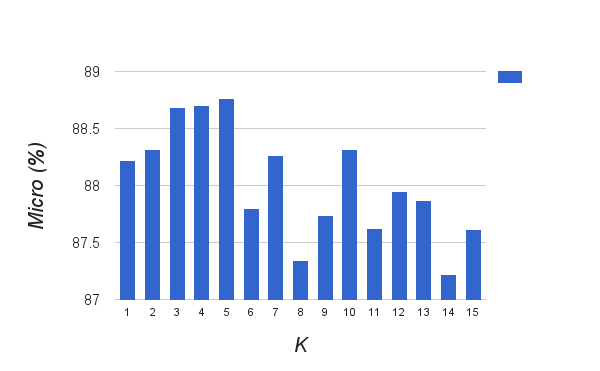
\includegraphics[width=\linewidth]{./k_effect.png}
\caption{Effect of parameter $K$ on entity linking accuracy.
Trained on CoNLL train and tested on CoNLL test-a.}
\label{fig:k_effect}
\end{figure}
}
% PGF plot version of the figure
{
\pgfplotsset{every tick label/.append style={font=\tiny}}
\begin{figure}[t!]
\centering
\resizebox {\columnwidth} {!} {
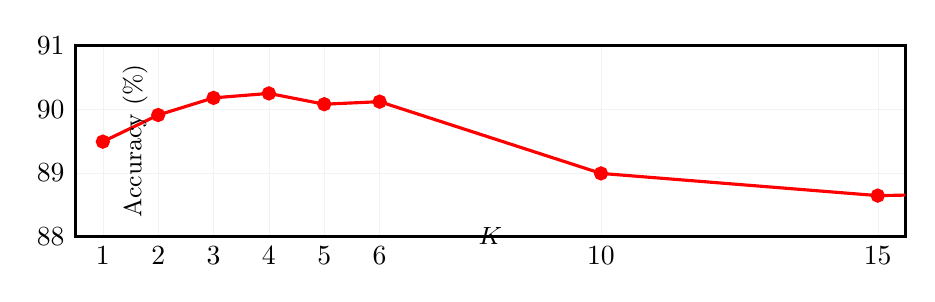
\begin{tikzpicture}
  \begin{axis}[
   %title  = Effect of K,
   width = \columnwidth,
   height=4cm,
%    ybar,
 %   bar width = 0.2cm,
    %x axis line style = { opacity = 0 },
    %axis y line       = none,
    tickwidth         = 0pt,
    xmin=0.5,xmax=15.5,
    ymin=88,ymax=91,
    grid=both,
    grid style={line width=.1pt, draw=gray!10},
    x label style={at={(axis description cs:0.5,0.1)},anchor=north},
    y label style={at={(axis description cs:0.1,.5)},anchor=south},
    xlabel={\small $K$},
    ylabel={\small Accuracy (\%)},
    mark size=2.0pt,
    line width=1.0pt,
   % enlarge y limits  = 0.2,
    xtick = data,
  ]
  \addplot [line width=0.4mm, red, mark=*, mark options=solid] coordinates { 
    (1,89.49) (2,89.91)  (3,90.18) (4,90.25) (5,90.08) (6,90.12) (10,88.99) (15,88.64) (20,88.72)
  };
  \pgfresetboundingbox
  %\addplot coordinates { (20,1)         (15,2)
   %                      (60,3)   (75,4)  };
 % \legend{Topics, Posts}
  \end{axis}
\end{tikzpicture}
}
\caption{Effect of parameter $K$ on entity linking accuracy.
Trained on CoNLL train and tested on CoNLL test-a. \label{fig:k_effect}}
\end{figure}
}

%(1,89.72) (2, 89.77) (3, 90.39) (4, 90.39) (5, 90.52)   (6,90) (7,90) (8,90) (9,90) (10,90)   (11,90) (12,90) (13,90) (14,90) (15,90)};


\subsubsection{Examples of gains (and losses)}


\comment{
\section{Conclusion}
\label{sec:End}

We have described two new approaches to modeling coherence for entity
resolution.  While most existing systems consider all relations
between entity candidates for a document to assign a coherence score
to a candidate, we use a novel attention mechanism to select the most
relevant relations.  Our experimental results support \hl{do they?}
the premise that the inclusion of all relations can hurt performance.
Our models improve the performance of a baseline system on three
evaluation benchmarks, and our best multi-focal attention model
achieves state-of-the-art results on standard benchmarks against
highly competitive recently built systems.
}


%%% Local Variables: ***
%%% mode:latex ***
%%% TeX-master: "main.tex"  ***
%%% tex-main-file: "main.tex"  ***
%%% End: ***
